\documentclass[a4paper, twoside, utf8]{ctexart}
\usepackage[fontset=Fandol]{ctex}
\usepackage{anyfontsize}
\usepackage{subcaption}
\usepackage{adjustbox}
\usepackage{algorithm}
\usepackage{longtable}
\usepackage{abstract}
\usepackage{amsfonts}
\usepackage{appendix}
\usepackage{booktabs}
\usepackage{enumitem}
\usepackage{fancyhdr}
\usepackage{geometry}
\usepackage{graphicx}
\usepackage{tabularx}
\usepackage{listings}
\usepackage{amsmath}
\usepackage{caption}
\usepackage{lipsum}
\usepackage{minted}
\usepackage{xcolor}
\usepackage{array}
\usepackage{url}

\geometry{a4paper,left=31mm,right=31mm,top=25mm,bottom=25mm}
\setlength{\parindent}{2em}
\ctexset{section = {format = \raggedright\large\bfseries}}
\let\oldsection\section
\renewcommand{\abstracttextfont}{\normalsize}

\pagestyle{fancy}
\fancyhf{}
\fancyhead[CO,CE]{议程管理系统 \ Agenda}
\fancyhead[LE]{编译器构造实验}
\fancyhead[RO]{Lab02设计文档}
\fancyhead[RE,LO]{}
\fancyfoot[CO]{\thepage}
\fancyfoot[CE]{\thepage}
\fancyfoot[LE,RE]{}
\fancyfoot[LO,RO]{}

\title{\songti \bfseries 议程管理系统 \ 设计文档}
\author{\fangsong 傅祉珏 \ \ 21307210}
\date{\fangsong 中山大学计算机学院\ 广东广州\ 510006}

\begin{document}
	
	\begin{titlepage}
		\centering
		\rule{\textwidth}{1pt}
		\vspace{0.02\textheight}
		
		{\LARGE \kaishu 编译器构造实验 \quad Lab02设计文档}
		
		\vspace{0.02\textheight}
		
		{\Huge \songti \bfseries 议程管理系统}
		
        \vspace{0.025\textheight}
        \rule{0.83\textwidth}{0.4pt}
        \vspace{0.05\textheight} 
        
        \begin{figure}[htbp]
            \centering
            
\includegraphics[width=8cm, height=8cm]{./figure/计院院徽.jpg}
        \end{figure}

        \vspace{0.05\textheight} 
        {\Large 课程编号:\textsc{DCS292}}

        \vspace{0.025\textheight} 
        {\Large 学生姓名:\textsc{傅祉珏}}

        \vspace{0.025\textheight} 
        {\Large 学生学号:\textsc{21307210}}

        \vspace{0.025\textheight} 
        {\Large 指导老师:\textsc{李文军\ 教授}}
 
        \vspace{0.025\textheight} 
        {\Large 项目截止日期:\textsc{2025年4月10日}}

        \vspace{0.05\textheight} 
        \vfill

        {\large \today}
        \vspace{0.1\textheight}
        \rule{\textwidth}{1pt}
    \end{titlepage}
	
    \pagenumbering{Roman}
    \setcounter{page}{1}
    \renewcommand{\abstractname}{\Large \textbf{引言}}
    \addcontentsline{toc}{section}{引言}
    \begin{abstract}
        本设计文档系统阐述了基于Java语言开发的命令行议程管理系统的架构设计与工程实现方案。系统严格遵循多层架构范式,构建了包含用户界面层(UI)、业务逻辑层(BLL)、数据管理层(DML)和数据持久层(DAL)的四级分层体系,通过模块化设计与接口隔离策略实现组件间的低耦合与高内聚特性。项目深度实践了面向对象编程的核心思想,在用户管理、会议调度等核心模块中运用封装、继承、多态机制,结合单例模式保障全局状态一致性,采用反射机制实现动态指令扩展,并基于责任链模式构建双层异常检测体系。

        在数据管理层面,系统设计了用户管理类与会议管理类作为核心控制器,通过单例模式确保全局数据访问入口唯一性,实现用户注册、会议冲突检测、时间合法性校验等复杂业务逻辑。数据持久化采用文本文件存储方案,通过用户IO类、会议IO类与会议编号生成器的协同工作,完成用户凭证、会议元数据及自增ID的本地化存储,支持系统状态的断点续用能力。交互层创新性地引入命令解析器与反射机制,实现"指令-实现类"的动态映射,构建可扩展的命令行操作体系。

        本实验不仅验证了分层架构在工程实践中的可行性,更通过异常处理、单元测试、日志追踪等质量保障手段,完整呈现了从需求分析到架构设计、从核心算法实现到系统集成的软件开发全流程。项目成果为后续编译原理实验中的词法分析器、语法树构建等复杂系统开发提供了可复用的工程框架与设计范式。
        
        \vspace{1em}
        \noindent{\textbf{\heiti 关键词:}多层架构设计,面向对象编程,数据持久化,反射机制,模块化工程实践。}
    \end{abstract}
    \newpage

    \addcontentsline{toc}{section}{目录}
    \begingroup
    \setcounter{tocdepth}{2}
    \renewcommand{\section}{
        \renewcommand{\raggedright}{}
        \ctexset{section/format = \centering\Large\bfseries}
        \oldsection
    }
    \tableofcontents
    \endgroup
    \newpage

    \pagenumbering{arabic}
    \setcounter{page}{1}
	
	\maketitle

    \section{项目概述}

    \subsection{项目背景}

    在 Lab01 实验中,我们已经初步习得了 Java 语言的基础语法以及面向对象程序设计的基本方法。本次实验的目的在于进一步深化对面向对象编程思想的理解,并通过实践活动巩固封装、信息隐藏、数据抽象和异常处理等机制。此外,本实验亦旨在引导我们掌握继承、运行时多态性、程序包、多层体系结构及设计模式等高级特性,为后续的编译原理实验奠定坚实的基础。

    本次实验的任务是开发一个基于命令行交互的议程管理系统。该系统采用 Java 语言进行实现,遵循面向对象的设计原则,以命令行方式提供会议日程管理功能。通过本实验,我们不仅能加深对 Java 语言的掌握,还能提升软件架构设计能力,培养良好的编码习惯和工程实践经验。

    \subsection{需求分析}

    议程管理系统的核心功能在于提供会议安排的管理服务,涵盖会议的创建、移除以及检索等基础操作。系统用户初始阶段需完成注册流程,注册成功后,用户得以在系统内构建会议日程,并执行相应的管理活动。此外,系统亦赋予用户能力,以清除其组织的所有会议安排。
    
    所有交互活动均通过命令行界面实现,不包含图形用户界面(GUI)设计元素。用户通过命令行界面输入预设格式的指令,系统解析输入并执行相应操作,如会议的添加、移除或查询。系统应具备错误处理机制,以应对非标准输入,确保交互过程的顺畅及系统的稳定性。

    \subsection{系统设计目标}

    本研究旨在构建一系统,其设计目标涵盖软件架构的合理性、系统的适应性、健壮性以及程序组织方式的优化。
    
    在软件架构层面,本系统至少应采纳双层架构模式,明确区分用户界面层(UI)与业务逻辑层(BLL),以提升系统的可维护性与可扩展性。同时,系统内部的类设计需遵循面向对象编程原则,确保模块间低耦合与高内聚,合理规划类接口,以促进代码复用。
    
    关于适应性,本系统应具备卓越的扩展性,以便于未来在不进行大规模代码重构的情况下添加新功能。系统组件应设计为尽可能通用,以支持在不同环境下的复用,从而增强软件的灵活性。
    
    在健壮性方面,系统需构建完善的异常处理机制,确保在用户输入错误命令或发生意外情况时,系统能即时提供反馈信息,并防止程序崩溃。同时,应保证数据存储与读取的稳定性,避免因异常情况导致数据损坏或遗失。
    
    为提高代码的可维护性和可读性,本系统应充分利用 Java 语言所提供的包(package)机制,对不同功能模块进行有效组织,实现代码结构的清晰化与层次化,为后续大型程序设计奠定坚实基础。

    \section{系统架构设计}

    \subsection{整体架构分层说明}

    本系统项目采用四级架构模式,涵盖用户界面层(UI)、业务逻辑层(BLL)、数据管理层(DML)以及数据持久层(DAL)。
    
    用户界面层(UI)承担与用户交互的职责,负责接收用户在命令行中输入的指令,并将相应的操作请求传递至系统。该层解析用户输入的命令,调用业务逻辑层执行对应的功能,并将操作结果反馈给用户。
    
    业务逻辑层(BLL)作为系统的核心,主要负责对会议和用户的抽象化处理,并实现相关业务逻辑功能。该层依据用户请求,执行会议的创建、移除、检索等操作,同时确保系统逻辑的完整性和一致性。
    
    数据管理层(DML)主要负责管理会议集合和用户集合,协调业务逻辑层与数据持久层之间的交互,保障数据的有效性和一致性。该层提供数据存取接口,并对数据生命周期进行管理。
    
    数据持久层(DAL)承担数据存储与持久化任务,确保系统重启后仍能使用先前保存的数据。会议数据和用户数据通过该层存储至文件系统,以实现数据的持久化。

    \begin{figure}
        \centering
        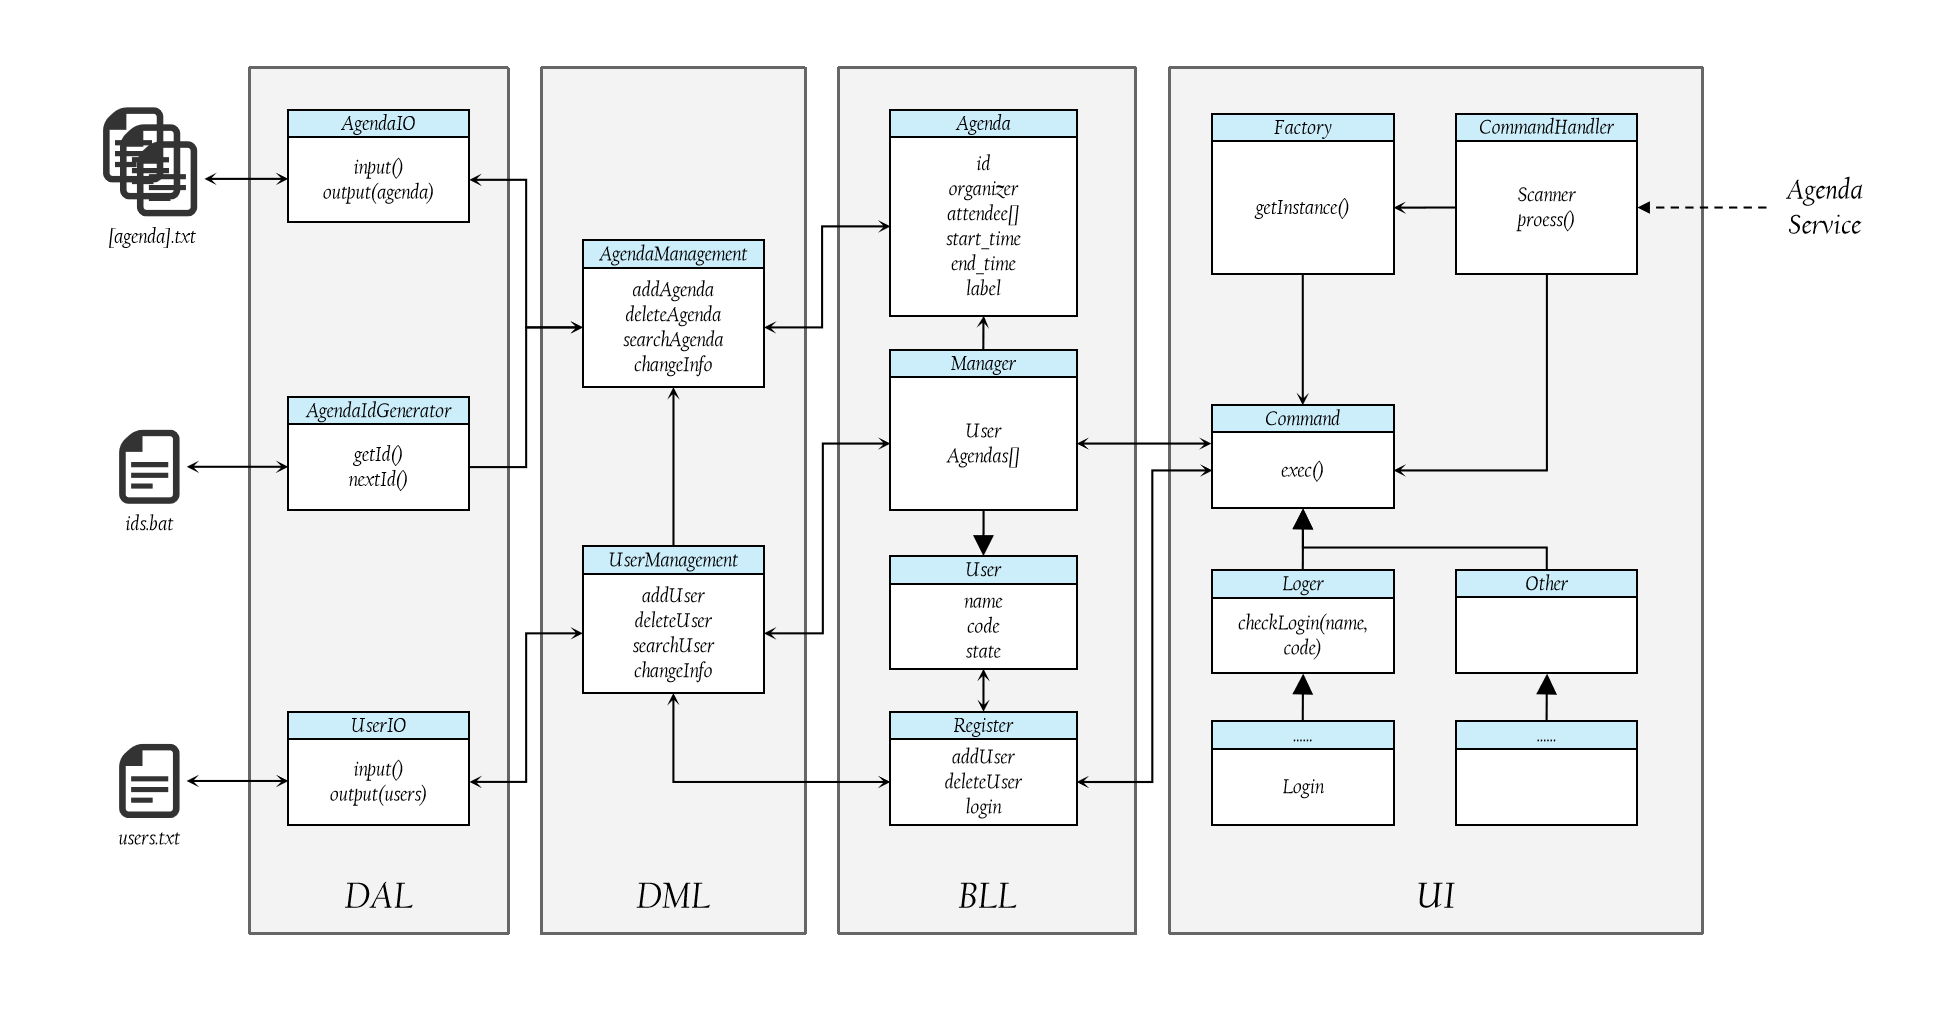
\includegraphics[width=.9\linewidth]{figure/structure.png}
        \caption{系统架构设计图}
    \end{figure}

    \subsection{各模块交互关系}

    本系统采用的四层架构严格遵循层次化设计原则,各层次间仅通过相邻层次进行交互,有效避免了跨层次的调用,从而确保了系统结构的清晰性与可维护性。
    
    系统启动伊始,用户在用户表示层输入指令,该层次负责解析指令并将其转化为相应的操作请求,传递至业务逻辑层。业务逻辑层对请求进行处理,并调用数据管理层以执行数据的存取与管理任务。数据管理层与数据持久层协同工作,确保数据的准确存储与高效读取。
    
    在系统运行期间,所有会议信息与用户信息由数据管理层负责维护,并通过数据持久层最终存储于文件系统中。系统重启时,数据持久层负责从磁盘加载数据,并将其返回给数据管理层,以恢复至上次会话的会议信息与用户数据状态。
    
    功能执行完毕后,数据管理层与业务逻辑层将执行结果反馈至用户表示层,并最终呈现给用户,从而完成整个交互流程。
    
    \section{业务逻辑层设计}

    \subsection{核心业务类设计}

    本系统的核心业务类涵盖用户类与会议议程类,二者构成了整个系统的核心抽象。

    用户类作为用户数据的抽象,包含用户名与密码属性。用户在注册过程中需设定唯一标识的用户名及作为登录凭证的密码。该类支持通过接口调用获取用户信息,实现用户名与密码的更新,以及对用户名的唯一性进行校验。

    会议议程类作为会议数据的抽象,包含组织者、与会人、开始时间、结束时间、标签及唯一标识的会议编号。会议编号作为唯一标识符,确保每个会议的编号唯一,包括已删除的会议,以防止编号重用导致数据混淆。该类支持通过接口调用获取会议详细信息,并允许修改会议组织者、添加或删除与会人、更改会议标签等操作。

    用户类与会议议程类均具备唯一标识符,因此可实现 \verb|Comparable| 接口以支持排序功能。用户类依据用户名的 Unicode 编码顺序排序,而会议议程类首先按会议时间排序,其次按编号排序。采用 \verb|Comparable| 接口的继承方式,便于后续数据集合操作的管理。

    \subsection{派生业务类设计}
    
    基于用户类与用户议程类,为满足特定操作需求,同时避免跨层调用接口,需派生出其他业务类作为用户表示层与数据管理层之间的桥梁。
    
    首先,会议管理员类继承自用户类,负责管理用户持有的会议。该类具备会议管理类的重复性操作,但需区分的是,数据管理层的会议管理类管理所有会议,而会议管理员类仅针对特定用户的会议进行管理。此设计有效隔离了用户访问非相关会议的数据,同时允许管理自身所属会议,实现数据隔离。会议管理员类还需实现会议的增删查改操作。
    
    其次,用户注册类不继承自会议议程类或用户类,无类变量,仅包含创建用户、注销用户及用户登录的方法,故命名为用户注册类。该类负责用户创建、注销及登录操作。尽管部分方法与用户管理类重复,但该类仅作为用户管理操作的接口,同时作为用户登录验证的依据。
    
    \section{数据持久层设计}
    
    \subsection{数据存储方案}
    
    为了简化数据持久层的操作设计,并将关注点着重注焦于核心功能的设计及用户的体验反馈上,本系统采用最为朴素的数据存储方案,即本地存储。通过文件系统及字节流传输方法,将程序中涉及到的数据转存入本地,并以 .txt 文件进行存储。
    
    基于前述整体设计思路,如需要进行数据持久化,则需要存储用户数据及各个会议的数据。由于用户数据较少,因此仅需要将所有的用户的用户名及其密码存储至同一文件当中。而由于会议数据所包含的子数据更多,且整体性更强,因此需要分别对每一会议的数据存储至一个文件当中,再将这些会议数据存储至同一文件夹中,以方便读取及管理。而先前提及,由于会议编号需要单调递增且不重复,因此也需要将该会议编号存储至一本地文件当中,以方便后期读取。由于会议编号不可更改,由系统自动生成,因此对于会议编号的存储不使用 \verb|.txt| 文件进行存储,而是使用 \verb|.bat| 文件进行存储。
    
    \subsection{持久化类设计}
    
    基于数据存储方案,该层设计由三个持久化类构成,分别为用户 IO 类,会议 IO 类及会议编号生成类。三个类分别完成三类数据的持久化实现。
    
    用户 IO 类用于完成对用户数据的持久化。用户 IO 类在存储用户数据的时候是对所有的用户进行统一存储。首先用户 IO 类通过用户管理类获取当前所存储的所有用户信息,并通过迭代器遍历所有的用户信息将其存储至文件当中。读取则直接读取存储所有用户信息的文件,并通过正则表达式分割用户信息,并将不同的用户信息读取回入用户管理类中进行操作。
    
    会议 IO 类用于完成对会议数据的持久化。根据前述数据存储方案,会议 IO 类分别对每一个 Agenda 进行单文件的存储,因此在此类当中仅仅实现对单个会议进行存储,而对所有会议进行存储的工作则交由会议管理类调用该方法进行实现。读取则一次性读取所有存储了会议的文件信息,并交由会议管理类进行分类及完成接下来的操作。
    
    由于会议的编号需要进行持久化的存储,因此另外设计了会议编号生成类完成该任务。会议编号生成类采取单例设计模式,即该类在整个程序的运行周期只允许实例化一次,这是为了避免实例化多次导致会议编号生成不一致或需要处理更多线程异常的情况发生。会议编号生成类可获取当前的会议编号,可将会议编号加 1 后获取,也可以将当前的会议编号减 1。同时该类可将当前的会议编号存储进文件系统中,并在系统启动时从文件系统当中读取当前的会议编号。这种做法不仅可以在会议添加失败时依旧保持当前的编号一致,同时也可以正常生成会议的编号。当文件系统当中的文件被删除,则编号从 0 重新开始重新计数。
    
    \section{数据管理层设计}

    \subsection{管理层功能说明}

    在议程管理系统中,数据管理层承担着连接业务逻辑层与数据持久层的中间枢纽作用,其核心目的是对程序中涉及到的各种数据进行有效管理与协调。由于系统涉及用户与会议两个主要的数据对象,若直接通过IO进行数据操作,不仅逻辑繁琐,耦合度高,而且极易出错。举例而言,当我们希望更改某一会议的组织者信息时,若缺乏统一管理机制,则需分别操作原组织者与新组织者的用户信息,并同步更新会议参与者列表,这一过程既冗杂又不可靠。

    因此,为简化操作并提升数据处理的效率与正确性,系统引入数据管理类对抽象出来的用户类与会议类进行集中管理。这些管理类不仅支持用户与会议对象的增删查改操作,同时还承担协调数据状态、维护数据一致性的重要职责。通过将所有业务对象纳入管理类的统一调度,系统避免了跨层调用或冗余操作,使得整体结构更清晰、逻辑更简洁。

    \subsection{数据管理类设计}

    数据管理层由两个核心管理类构成:用户管理类和会议管理类,分别用于管理所有系统中的用户数据和会议数据。考虑到这些管理类在整个程序运行周期中仅需保持一个全局实例以维护系统状态的一致性,因此采用单例模式进行设计,确保在任意时刻,系统中只存在一个用户管理器和一个会议管理器。

    用户管理类提供用户对象的增、删、查、改操作。在添加用户时,管理类首先校验用户名的唯一性,若发现重复用户名则添加失败,并返回相应的错误提示或错误码;删除用户则同时需要清除与该用户相关联的所有会议安排,以避免数据冗余或数据孤岛的产生;修改用户信息操作也在管理类内实现,确保变更后的用户状态同步反映在整个系统中。

    会议管理类负责对所有会议对象进行集中管理,同样支持会议的新增、删除、查询和修改操作。相较于用户管理类,会议管理类在功能实现上更为复杂,因为其操作不仅涉及会议对象本身的数据变更,还需维护与用户对象之间的绑定关系,以及对会议时间的合法性进行校验。在新增会议时,系统将首先判断新会议是否与当前用户已有的会议产生时间冲突;在删除会议时,需同步更新与会人员的相关数据状态;而会议的修改操作也必须确保在更改任何会议属性(如组织者、时间、标签)时不会破坏系统的数据一致性。

    \section{用户交互层设计}

    \subsection{命令处理机制}

    本系统采用命令行交互方式,因此在用户交互层的设计中,命令的解析与执行机制显得尤为关键。系统主方法采用循环结构实现,其核心逻辑是持续监听用户输入,直到用户主动发出退出指令。每次循环中,系统首先接收用户输入的原始字符串,随后调用命令解析模块将其解析为命令名称及参数集合。解析完成后,系统依据命令名称识别对应的命令类,并将参数传入该类完成命令的具体业务逻辑处理。整个处理过程遵循“输入 $\rightarrow$ 解析 $\rightarrow$ 匹配 $\rightarrow$ 执行”的流水式逻辑,使得系统结构清晰、扩展性强。此外,命令的解析过程考虑了用户输入的灵活性,例如参数的前后顺序、空格的容忍度等,确保系统具有良好的用户友好性。

    \begin{figure}[htbp]
        \centering
        \begin{minipage}{.45\textwidth}
            \centering
            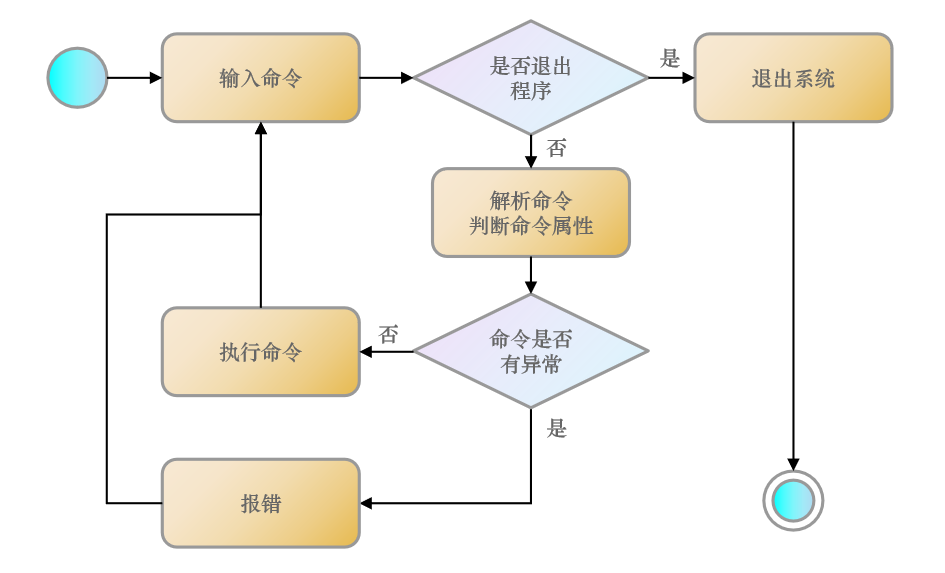
\includegraphics[width=.9\linewidth]{figure/process.png}
            \caption{用户交互过程}
        \end{minipage}
        \begin{minipage}{.45\textwidth}
            \centering
            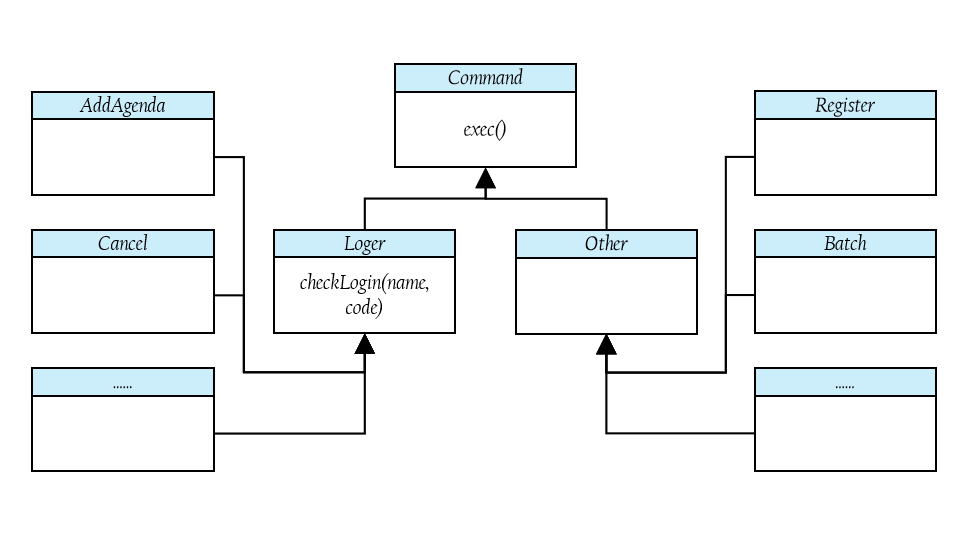
\includegraphics[width=.9\linewidth]{figure/command.png}
            \caption{指令类继承模式}
        \end{minipage}
    \end{figure}

    \subsection{反射机制}

    为了提升系统的可扩展性和指令功能的灵活性,命令类的设计采用了反射机制。反射机制是一种在运行时动态获取类信息并进行操作的能力,允许系统在不显式调用具体类名的情况下,根据输入动态实例化并调用类中的方法。在本系统中,我们首先设计了统一的指令接口,该接口定义了所有命令类需实现的执行方法。所有的命令类无论是否依赖用户登录状态,都实现了该接口,从而保证调用方式的一致性。

    在命令处理过程中,系统通过命令解析器提取用户输入的命令名称,并将该名称转换为对应的类名,然后通过 Java 的反射机制动态创建该类的实例,并调用其执行方法。由于指令类的生成与系统主结构解耦,开发者在新增功能时只需新增一个实现指令接口的类并命名为符合规则的命令类,即可被系统自动识别并调用,极大地简化了系统的维护与扩展过程,体现出良好的面向对象设计思想。

    \subsection{异常处理机制}

    在用户交互过程中,异常处理机制是保障系统健壮性与用户体验的关键手段。为了更全面地覆盖各类可能出现的异常情况,系统在命令处理流程中引入了双层异常检测机制。

    第一层为输入阶段的异常检测,主要负责识别用户输入格式是否符合规范。例如,当用户输入了一个不存在的指令,或在命令参数中使用了非法的数字格式、错误的日期格式等,系统会在命令解析阶段及时捕获异常,并输出明确的错误信息提示用户纠正输入。第二层为命令执行阶段的异常处理,它关注的是逻辑层面的问题,如用户尝试使用错误的密码登录、创建重复用户名的用户、创建时间冲突的会议等逻辑冲突。这一层的异常会在命令类的执行方法中通过逻辑判断主动抛出,再由系统捕获并输出相应的提示信息。

    通过这两层异常检测机制的协同工作,不仅保证了系统在输入格式和逻辑功能层面的健壮性,也通过友好的提示信息引导用户纠正错误操作,提升了整个系统的可用性与交互体验。
	
    \addcontentsline{toc}{section}{参考文献}
    \begin{thebibliography}{99}
        \bibitem{ref1} 沐言科技\ 李兴华.\ Java编程\ 从入门到实践[M].\ 第1版.\ 安徽:中国水利水电出版社,\ 2021.
        \bibitem{ref2} 毛新军,\ 董威.\ 软件工程——理论与实践[M].\ 第1版.\ 北京:高等教育出版社,\ 2024.
    \end{thebibliography}
	
	\newpage
	\appendix
	\centerline{\Large{\textbf{附录}}}

    \section{用户功能手册}

    \begin{center}
        \setlength{\LTcapwidth}{\textwidth}
        
        \small
        
        \begin{longtable}{
            >{\centering\arraybackslash}m{.2\textwidth}
            | >{\raggedright\arraybackslash}m{.7\textwidth}
        }
            
            \toprule
            \multicolumn{1}{c|}{\textbf{指令}} & \multicolumn{1}{c}{\textbf{用法}} \\
            \midrule
            \endfirsthead
            
            \multicolumn{2}{l}{\footnotesize 续表} \\
            \toprule
            \multicolumn{1}{c|}{\textbf{指令}} & \multicolumn{1}{c}{\textbf{用法}} \\
            \midrule
            \endhead
            
            \midrule
            \multicolumn{2}{r}{\footnotesize 接下页}
            \endfoot
            
            \bottomrule
            \endlastfoot

            \verb|help| & View all available commands \\
            \verb|register| & Register a new user \\
            \verb|cancel| & Cancel an existing user \\
            \verb|rename| & Rename the current user \\
            \verb|recode| & Reset the current user's password \\
            \verb|addagenda| & Add a agenda \\
            \verb|deleteagenda| & Delete a specified agenda \\
            \verb|clearagenda| & Clear all agendas hosted by the current user \\
            \verb|queryagenda| & Query specified agendas \\
            \verb|addattendee| & Add a attendee to a specified agenda \\
            \verb|deleteattendee| & Remove a attendee from a specified agenda \\
            \verb|changeorganizer| & Change an organizer from a specified agenda \\
            \verb|batch| & Execute a batch of commands from a text file \\
            \verb|developer| & Check the developers of this system \\
            \verb|quit| & Exit the system \\
            
        \end{longtable}
        \vspace{-3em}
    \end{center}

    \section{用户指令手册}

    \begin{center}
        \setlength{\LTcapwidth}{\textwidth}
        
        \small
        
        \begin{longtable}{
            >{\raggedright\arraybackslash}m{.93\textwidth}
        }
            
            \toprule
            \multicolumn{1}{c}{\textbf{指令格式}} \\
            \midrule
            \endfirsthead
            
            \multicolumn{1}{l}{\footnotesize 续表} \\
            \toprule
            \multicolumn{1}{c}{\textbf{指令格式}} \\
            \midrule
            \endhead
            
            \midrule
            \multicolumn{1}{r}{\footnotesize 接下页}
            \endfoot
            
            \bottomrule
            \endlastfoot

            \verb|help| \\
            \verb|register [userName] [password]| \\
            \verb|cancel [userName] [password]| \\
            \verb|rename [userName] [password] [newName]| \\
            \verb|recode [userName] [password] [newCode]| \\
            \verb|addagenda [userName] [password] [attendee] [starttime] [endtime] [label]| \\
            \verb|deleteagenda [userName] [password] [agendaID]| \\
            \verb|clearagenda [userName] [password]| \\
            \verb|queryagenda [userName] [password] [starttime] [endtime]| \\
            \verb|queryagenda [userName] [password] [agendaID]| \\
            \verb|queryagenda [userName] [password]| \\
            \verb|addattendee [userName] [password] [agendaID] [attendee]| \\
            \verb|deleteattendee [userName] [password] [agendaID] [attendee]| \\
            \verb|changeorganizer [userName] [password] [agendaID] [organizer]| \\
            \verb|batch [fileName]| \\
            \verb|developer| \\
            \verb|quit| \\
            
        \end{longtable}
        \vspace{-3em}
    \end{center}
	
\end{document}
